\documentclass[pdftex, a4paper]{scrartcl}
\usepackage{ngerman}
\usepackage[utf8]{inputenc}
\usepackage[T1]{fontenc}
%\usepackage{array}
%\usepackage{subfiles}
\usepackage{url}
\usepackage[hidelinks]{hyperref}
\usepackage{parskip}
\setlength{\parskip}{1em}
\usepackage{xurl}
\usepackage[nottoc,notlot,notlof]{tocbibind}
\usepackage{longtable}
\usepackage{setspace}
\linespread{1.5}
% \usepackage[
% top    = 2.75cm,
% bottom = 2.50cm,
% left   = 3.00cm,
% right  = 2.50cm]{geometry}
\usepackage{etoolbox}
\AtBeginEnvironment{thebibliography}{\linespread{1}\selectfont}
\usepackage{endnotes}
\interfootnotelinepenalty=10000
\usepackage[acronym,toc,sort=def]{glossaries} 
\usepackage[titletoc]{appendix}
\usepackage{booktabs}
\usepackage{tabularx}
\usepackage{graphicx}
\usepackage{textcomp}
\usepackage{lscape}
\usepackage{fancyhdr} 
\usepackage{multirow}
\usepackage{caption}
\usepackage{natbib}
\usepackage[table,xcdraw]{xcolor}
\usepackage{float}
%\usepackage{lineno}
\usepackage{longtable}
\usepackage{tabularx}
\renewcommand\tabularxcolumn[1]{m{#1}}
\usepackage{enumitem}
\usepackage{spverbatim}

\makeglossaries
\loadglsentries{0.2_Glossar}

% &as_qdr=y2 (find date)

\fancypagestyle{lscape}{
\fancyhf{} %Clears the header/footer
\fancyfoot{% Footer
\makebox[\textwidth][r]{% Right
  \rlap{\hspace{1cm}% Push out of margin by \footskip
    \smash{% Remove vertical height
      \raisebox{4.87in}{% Raise vertically
        \rotatebox{90}{\thepage}}}}}}% Rotate counter-clockwise
\renewcommand{\headrulewidth}{0pt}% No header rule
\renewcommand{\footrulewidth}{0pt}% No footer rule
}

\begin{document}
  \begin{titlepage}
    \vspace*{2mm}
    \begin{center}
        \Large
        \textbf{Hochschule Worms}\\
        \textbf{Fachbereich Informatik}\\
        \textbf{Studiengang Angewandte Informatik B.Sc.}\\
        \vspace{3cm}
        \textbf{TBD}\\
        \vspace{1cm}
        \large
        Bacherloarbeit xxx\\
        \vspace{3cm}
        \begin {table}[ht]
        \centering
            \begin{tabular}{c}
                Bruno Macedo da Silva  \\ 
                676839                \\
                inf3645@hs-worms.de   \\
                Bebelstraße 22 Z10    \\
                67549 Worms            \\
            \end{tabular}
        \end {table}
        \vspace{2cm}
        \large
        \vspace{1cm}
        \begin{table}[h]
            \centering
            \begin{tabular}{l l}
                \multirow{2}{*}{Betreuer} & Prof. Dr. Zdravko Bozakov \\
                Bearbeitungszeitraum:     & Sommersemester 2023 \\
                Abgabedatum:              & xx. xxx 2023 \\
                Sperrvermerk:             & Ja/Nein \\
            \end{tabular}
        \end{table}    
    \end{center}
    \normalsize
    \vfill
\end{titlepage}
  \tableofcontents
  \newpage
  \phantomsection
  \addcontentsline{toc}{section}{Abstract}
  \begin{abstract}

    \begin{center}
        \textbf{Abstract}
    \end{center}

%This thesis has as goal to use an \gls{opensource} similar \glsfirst{SIEM} tool to monitor security events. Most of the existing \glsplural{SIEM} solutions are either \gls{Proprietary} or have only limited free features. For that we decide to implement our monitoring system using Grafana and its integrated elements: Promtail, Loki and Alerting. Grafana is primarly used to generate graphics based on the user's input. In our study, we used \gls{ssh} log files as input. The files were extracted by Promtail from the \glsplural{Endpoint} and sent to Loki which aggregates them and filters their content based on the rules defined to identify possible cyberatacks against a \gls{ssh} Server. Once the searched information was extracted, it was sent to Grafana to generate an visually overview about the \gls{ssh} connections. Eventually we used the tool Alerting to send notifications about pottentially attacks identified in our rules. The recognition of the possible attack and the ruleset used was based on the description provided by \gls{mitre} Matrix. The combined use of the aforementioned tools proved to be realiable, affordable and usefull to detect static base attacks. The main burdens of using these tools as a replacement to a \gls{SIEM} solution would be: the properly definition of the ruleset used to read and extract information about cyberattacks from the log files; and adapting those rules to scerarios where attacks have more dynamic flows.

%The goal of this thesis is to use an \gls{opensource}, similar tool to a \glsfirst{SIEM} system for monitoring security events. Most of the existing \glsplural{SIEM} solutions are either proprietary or have limited free features. Therefore, we decided to implement our monitoring system using Grafana and its integrated elements: Promtail, Loki, and Alerting. Grafana is primarily used to generate graphics based on user input. In our study, we used \gls{ssh} log files as input. Promtail extracted the files from the \glsplural{Endpoint} and sent them to Loki, which aggregated and filtered their content based on defined rules to identify possible cyberattacks against an \gls{ssh} server. Once the information was extracted, Grafana was used to generate a visual overview of the \gls{ssh} connections. We used the Alerting tool to send notifications about potential attacks identified by our rules. The recognition of possible attacks and the ruleset used was based on the descriptions provided by the \gls{mitre} Matrix. The combined use of these tools proved to be reliable, affordable, and useful in detecting static-based attacks. The main challenges of using these tools as a replacement for a \gls{SIEM} solution would be properly defining the ruleset used to read and extract information about cyberattacks from log files and adapting those rules to scenarios where attacks have more dynamic flows.

The aim of this thesis is to develop a reliable, cost-effective solution for monitoring security events by utilizing an \gls{opensource}, \gls{SIEM}-like tool. Since many existing \gls{SIEM} solutions are either proprietary or offer limited free features, we chose to use Grafana and its integrated tools - Promtail, Loki, and Alerting - to create our monitoring system. Grafana is primarily used to generate customizable graphics based on user input, and in our study, we used \gls{ssh} log files as input. Promtail extracted the files from \glsplural{Endpoint} and sent them to Loki, which used defined rules to aggregate and filter the content in order to identify possible cyberattacks against an \gls{ssh} server. Once the information was extracted, Grafana was used to provide a visual overview of the \gls{ssh} connections. Additionally, we employed the Alerting tool to send notifications about potential attacks identified by our rules. The ruleset we used to recognize potential attacks and the descriptions of these attacks were based on the \gls{mitre} Matrix. We found that the combined use of these tools was reliable, affordable, and useful for detecting static-based attacks. The main challenges in using these tools as a replacement for a \gls{SIEM} solution are properly defining the ruleset used to read and extract information about cyberattacks from log files and adapting those rules to scenarios where attacks have more dynamic flows.


\vspace{3cm}
\textbf{Keywords: Monitoring Tool, Grafana Loki Cyberattacks,\gls{SIEM}}


\end{abstract}
  \addcontentsline{toc}{section}{\listfigurename}
  \listoffigures
  \clearpage
  \printglossary[title=Glossar,toctitle=Glossar]
  \clearpage
  \newpage
  \clearpage
  \begin{singlespacing}
    \printglossary[type=acronym,title=Abkürzungsverzeichnis,toctitle=Abkürzungsverzeichnis, nonumberlist, nogroupskip]
  \end{singlespacing}
  \clearpage
  \section{Einleitung}

Der heutige Netzwerkverkehr ist fast tausendfach größer als vor 20 Jahre \citep{Roser_I}. Das Internet wird heutzutage für fast all unsere Tätigkeiten verwendet: Soziale Netzwerke, Video und Audio-Streaming, Einkauf, behördliche Angelegenheiten und viele andere. So viel Verkehr generiert eine unermessliche Menge von Daten, die alle möglichen Inhalte beinhalten, von unschuldigen Anfragen nach einem eigenen Kontostand bis zur Ausführung von beabsichtigten Anfragen, um Systeme lahmzulegen. Um ersteres vom letzterem zu unterscheiden, verwenden viele Firmen das sogenannte \glsfirst*{SIEM} oder Log-Analyse-Tools. 

Das \glsfirst{NIST} definiert \gls{SIEM} als Software für die Sammlung, Anpassung, Analyse, Überwachung und Bedrohungserkennung von Sicherheitsdaten aus verschiedenen Quellen \citep{NIST_Definitions}. Die Bewertung dieser Daten spielt eine wesentliche Rolle bei solchen Anwendungen, um zu entscheiden, ob es sich um legitime Anfrage oder um einen \glsplural{Cyberangriff} handelt. Mit den Daten von \gls{SIEM} kann das \glsfirst{SOC} Team Maßnahmen ergreifen. Log Analysis und Log Management beziehen sich auf die Sammlung, Bearbeitung, Speicherung und/oder Löschen, Weiterleitung und Überwachung von Loginformationen. In dieser Arbeit benutzen wir den Begriff \quotes{Log-Analyse-Tools}, um diese Systeme zu referenzieren.

In diesem Projekt recherchieren und vergleichen wir existierende \gls{SIEM} und Log-Analyse-Tools. Danach entscheiden wir uns für eine \gls{opensource} Lösung, um eine kostengünstige Verbreitung und Implementierung zu ermöglichen. Mit dem ausgewählten Tool analysieren und bewerten wir spezifische Logdateien, damit wir demnächst potenzielle Angriffe erkennen können. Die Regelsätzen für die Angriffserkennung sollen mithilfe der \glsfirst{ttp} von \gls{mitre} aufgebaut werden.

\newpage
Unser Ziel ist es, eine umfangreiche \gls{opensource} Lösung zu finden bzw. zu gesltaten, die uns ermöglicht, \glsplural{Cyberangriff} nach vordefinierten Regelsätzen zu detektieren. \glsplural{Proprietary} Lösungen gibt es viele auf dem Markt. Sie sind meistens kostenpflichtig und verlangen spezielle Wartung. Da sich solche Lösungen eher an große Konzerne richten, beschäftigen wir uns mit dem Aufbau und Strukturierung einer eigenen Lösung mithilfe von \gls{opensource} Tools. 

Diese Arbeit wird in folgende Teile geteilt: 

% OSSIN: https://sourceforge.net/projects/os-sim/
% Preludes: https://www.prelude-siem.org/projects/prelude/wiki/ManualUser
% ELK Stack

% Grafana / Promtail: https://grafana.com/products/enterprise/
%https://grafana.com/logs/% 

%https://www.ossec.net/         https://github.com/ossec/ossec-rules

% was machen sie konkrent? / Vergleich zwischen OpenSource/Proprietary/

{\setstretch{1.5}
\begin{itemize}[noitemsep]
   \item	Definition von SIEMs und Log-Analyse-Tools 
   \item	Beschreibung von existierenden \gls{Proprietary}en und Open Source Lösungen
   \item	Entscheidung für die Implementation von einer Open Source Lösung
   \item Generierung und Extrahierung von Logdateien nach der Ausführung von einem ausgewählten \gls{Cyberangriff} 
   \item	Installation, Konfiguration und Generierung von Warnmeldungen mit den ausgewählten Anwendungen 
   \item	Definition der \gls{usecases} und Implementierung der Regelsätze für die Erkennung der vorherigen Angriffen anhand der \glsfirst{ttp} der \gls{mitre} Matrix 
   \item	Auswertung der implementierten Tools mit der Verwendung von  spezifischen Logdateien der Hochschule in der ausgewählten Lösung
\end{itemize}
}

\subsection{Problemstellung}
Während der Entwicklung dieser Arbeit beschäftigen wir uns mit folgenden Fragenstellung: 

{\setstretch{1.5}
% Regeln anhand mittre, automatisieren
\begin{itemize}[noitemsep]
   \item Wie können wir ein Log-Analyse-Tool konfigurieren, dass es vordefinierte Angriffe nach der \gls{mitre} Matrix automatisch erkennen kann? 
   \item Wie können wir allgemeine Regelsätze definieren, sodass wir sie später für die verschiedene \gls{ttp} der \gls{mitre} Matrix nanpassen können?
\end{itemize}
}

\newpage
Das folgende Diagramm, \ref{fig:AblaufderArbeit}, stellt den Aufbau und Entwicklung dieser Arbeit dar, wie oben beschrieben:
% Diagram anpassen mit korrenkten Zielen

\begin{figure}[H]
   \centering
   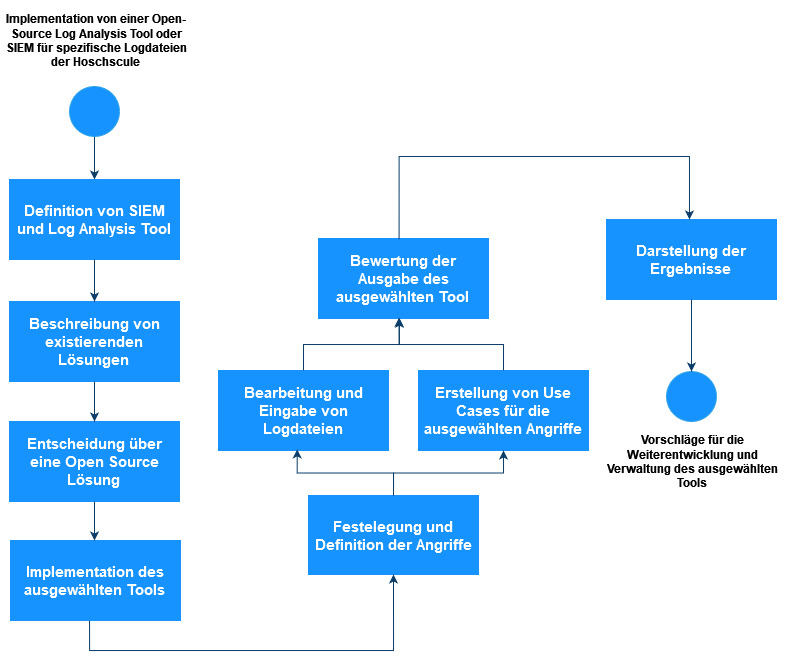
\includegraphics[width=1\textwidth]{assets/1_p1.jpg}
   \caption[Aufbau dieser wissenschaftlichen Recherche]
   {Aufbau dieser wissenschaftlichen Recherche \\Quelle: Eigene Darstellung }
   \label{fig:AblaufderArbeit}
   \centering
\end{figure}




  \section{Problemstellung}

Während der Entwicklung dieser Arbeit wollen wir uns mit folgenden Fragen beschäftigen:

\begin{itemize}
   \item Welche Information-Muster muss von dem \gls{SIEM} extrahiert werden, um Angriff\_1 und Angriff\_2 zu erkennen?
   \item Wie kann eine skript-basierte Lösung spezifische Daten extrahieren und bewerten, um Angriff\_1 und Angriff\_2 
\end{itemize}

% \begin{itemize}
%    \item Welche Information-Muster muss von dem \gls{SIEM} extrahiert werden, um Angriff_1 und Angriff_2 zu erkennen?
%    \item Wie kann eine skript-basierte Lösung spezifische Daten extrahieren und bewerten, um Angriff_1 und Angriff_2 zu identifizieren?
% \end{itemize}
  \section{Fazit}

Zuammenfassung der Zielen und der Ergebnissen.


  \nocite{*}
  \begingroup
    \setlength{\bibsep}{4pt}
    \setstretch{1}
    \bibliography{9_Referenzen}
    \endgroup
  \bibliographystyle{apalike}
 % \setcitestyle{authoryear, open={\(},close={\)}
  %\newpage
    
\end{document}


% &as_qdr=y2